\documentclass{article}
\addtolength{\oddsidemargin}{-1.cm}
\addtolength{\textwidth}{2cm}
\addtolength{\topmargin}{-2cm}
\addtolength{\textheight}{3.5cm}
  \usepackage[utf8]{inputenc}
  \usepackage{titlesec}
  \usepackage[pdftex]{graphicx}
  \usepackage{natbib}
  \setcounter{secnumdepth}{4}

  \newcommand\tab[1][1cm]{\hspace*{#1}}

  \title{\textbf{System Requirements and \\Design Documentation}\\
        \textbf{Group name:} Cerebero\\
       \textbf{ Project name:} eCivix Election Simulator}

  \date{May 2017}

 
  \author{Cerebero}
  \title{Election Simulator}

  \begin{document}

 % generates the Cover page	
  \begin{titlepage}
	
	\begin{center}
		% Upper part of the page       
		
\includegraphics[width=0.7\linewidth]{Images/uniLogo.jpg}\\
		% Title
		\rule{\linewidth}{0.5mm} \\[0.5cm]
		{ \huge \bfseries Tests and Reports}\\[0.3cm]
		{ \huge \bfseries Cerebero}\\[0.3cm]
		
\includegraphics[width=0.2\linewidth]{Images/cerebero.png}\\
		\rule{\linewidth}{0.6mm} \\[0.5cm] 		
  
		
		\begin{minipage}{0.4\textwidth}
			\begin{flushleft} \large
				Frederick Ehlers 
			\end{flushleft}
		\end{minipage}
		\begin{minipage}{0.4\textwidth}
			\begin{flushright} \large
				11061112
			\end{flushright}
		\end{minipage} \\[0.2cm]

		\begin{minipage}{0.4\textwidth}
			\begin{flushleft} \large
				 Jacobus Marais
			\end{flushleft}
		\end{minipage}
		\begin{minipage}{0.4\textwidth}
			\begin{flushright} \large
				15188397 
			\end{flushright}
		\end{minipage}\\[0.2cm]

		\begin{minipage}{0.4\textwidth}
			\begin{flushleft} \large
				Rikard Schouwstra
			\end{flushleft}
		\end{minipage}
		\begin{minipage}{0.4\textwidth}
			\begin{flushright} \large
				15012299
			\end{flushright}
		\end{minipage} \\[0.2cm]
		
		\begin{minipage}{0.4\textwidth}
			\begin{flushleft} \large
				Victor Twigge 
			\end{flushleft}
		\end{minipage}
		\begin{minipage}{0.4\textwidth}
			\begin{flushright} \large
				10376802
			\end{flushright}
		\end{minipage}\\[0.2cm]
		
		\rule{\linewidth}{0.5mm} \\[0.5cm] 
		{ \huge \bfseries Stakeholders}\\[0.3cm]	
		\rule{\linewidth}{0.2mm} \\[0.5cm] 
		\begin{minipage}{0.4\textwidth}
			\begin{flushleft} \large
				\emph{} \\
				Computer Science Department of University of Pretoria:
			\end{flushleft}
		\end{minipage}
		\begin{minipage}{0.4\textwidth}
			\begin{flushright} \large
				\emph{} \\
				Vreda Pieterse
			\end{flushright}
		\end{minipage}\\[0.2cm]

		\rule{\linewidth}{0.2mm} \\[0.5cm] 
		\begin{minipage}{0.4\textwidth}
			\begin{flushleft} \large
				\emph{} \\
				eCivix
			\end{flushleft}
		\end{minipage}
		\begin{minipage}{0.4\textwidth}
			\begin{flushright} \large
				\emph{} \\
				Daniël Eloff {Chairperson}
			\end{flushright}
		\end{minipage}
		\rule{\linewidth}{0.2mm} \\[0.5cm] 
		
	\end{center}
\end{titlepage}

  \tableofcontents
  \newpage

  \section{Functional Requirements}
  [Describe functional requirements of System.]
   \subsection{Game Play}
   	\begin{itemize}
   		\item Create User/Party
			\begin{itemize}
				\item Select and Customise the person/party that the player will be in the game
				\item Preconditions
				\begin{itemize}
					\item Registered and logged into their account
				\end{itemize}
				\item Post-conditions
				\begin{itemize}
					\item Started the game
				\end{itemize}
			\end{itemize}
	\end{itemize}
	
	\begin{itemize}
   		\item Select issues that the party supports
			\begin{itemize}
				\item Select which issues the party supports and how they feel about them.
				\item Preconditions
				\begin{itemize}
					\item Selected a party that they belong to
				\end{itemize}
				\item Post-conditions
				\begin{itemize}
					\item Calculates how much supporters you have in each province based on statistics
					\item Starts main game and begins the first round
				\end{itemize}
			\end{itemize}
	\end{itemize}
	
	\begin{itemize}
   		\item  Start Fund raising
			\begin{itemize}
				\item Start collecting funds nationally to campaign provincially 
				\item Preconditions
				\begin{itemize}
					\item User turn started.
				\end{itemize}
				\item Post-conditions
				\begin{itemize}
					\item Got funds to campaign
				\end{itemize}
			\end{itemize}
	\end{itemize}
	
	\begin{itemize}
   		\item  Polling
			\begin{itemize}
				\item Poll to check how good support is in that province
				\item Preconditions
				\begin{itemize}
					\item Have enough national funds to poll in the province.
				\end{itemize}
				\item Post-conditions
				\begin{itemize}
					\item See more or less how many supporters you have in that province.
				\end{itemize}
			\end{itemize}
	\end{itemize}
	
	\begin{itemize}
   		\item  Campaigning
			\begin{itemize}
				\item Campaign in a province to gather support
				\item Preconditions
				\begin{itemize}
					\item Have enough national funds to campaign in the province.
					\item The province should have been polled.
				\end{itemize}
				\item Post-conditions
				\begin{itemize}
					\item Gather or lose supporters based on how your campaign went.
				\end{itemize}
			\end{itemize}
	\end{itemize}
	
	\begin{itemize}
   		\item  Ending turn
			\begin{itemize}
				\item Ends the turn and allows AI to play their round
				\item Preconditions
				\begin{itemize}
					\item User is satisfied with what they have done in their turn
				\end{itemize}
				\item Post-conditions
				\begin{itemize}
					\item AI gets their turn.
				\end{itemize}
			\end{itemize}
	\end{itemize}
	
	\begin{itemize}
   		\item  Ending game
			\begin{itemize}
				\item The game has ended.
				\item Preconditions
				\begin{itemize}
					\item The date of the election has arrived.
				\end{itemize}
				\item Post-conditions
				\begin{itemize}
					\item The winner of the election is announced.
				\end{itemize}
			\end{itemize}
	\end{itemize}	
	\begin{itemize}
		\item Awarding man power for an action
			\begin{itemize}
				\item Users are awarded man power for doing campaigns 
				\item Preconditions
				\begin{itemize}	
					\item A campaign was completed before the end of the game
				\end{itemize}
				\item Post-conditions
				\begin{itemize}	
					\item Based on user's party preferences the effectiveness of the campaign is calculated.
					\item The calculated value is then added to the user's total man power.
				\end{itemize}
			\end{itemize}
	\end{itemize}
	\item Artificial Intelligence
	\begin{itemize}
			\begin{itemize}
				\item An intelligent agent that can play against the user to try and win the election
				\item Preconditions
				\begin{itemize}
					\item Game started
				\end{itemize}
				\item Post-conditions
				\begin{itemize}
					\item Game ended
				\end{itemize}
			\end{itemize}
	\end{itemize}
	\begin{itemize}
		\item Leader-board
			\begin{itemize}
				\item Display the user's position on the leader-board.
				\item Preconditions
				\begin{itemize}	
					\item The game has ended.
				\end{itemize}
				\item Post-conditions
				\begin{itemize}	
					\item User was able to view his position on the leader-board.
				\end{itemize}
			\end{itemize}
	\end{itemize}
	
   	\subsection{User management} 
    \begin{itemize}
    				\item Register as user or admin
				\begin{itemize}
					\item Use your personal details to register on system in order to gain access to more of the applications features.

					\item Preconditions
					\begin{itemize}
						\item Submit details on registration form
					\end{itemize}
					\item Post-conditions
					\begin{itemize}
						\item A personal account and profile is created for the user on the system
					\end{itemize}
				\end{itemize}
				
				\item Login
				\begin{itemize}
					\item Query user’s valid details on the system’s database through the login page to gain access to the account. 
					\item Preconditions
					\begin{itemize}
						\item Have to be registered on eCivix Election Simulator
						\item Have to submit his/her correct details on the login page
					\end{itemize}
					\item Post-conditions
					\begin{itemize}
						\item The user is redirected to their profile
						\item Have access to user features
					\end{itemize}
				\end{itemize}
				
				\item Admin manage user accounts
				\begin{itemize}
					\item User management is necessary if a user experiences problems with their password or any account related issues.
					\item Preconditions
					\begin{itemize}
						\item Have admin account and therefore rights
						\item Have internet access
						\item A management system in place
					\end{itemize}
					\item Post-conditions
					\begin{itemize}
						\item Users’ account related problems can be solved
					\end{itemize}
                \end{itemize}
           
			
				\item Edit profile information
				\begin{itemize}
					\item Allow users to add a summary and personal information. Also create provision for the use of a username for anonymity.
					\item Preconditions
					\begin{itemize}
						\item Submit information to the server
					\end{itemize}
					\item Post-conditions
					\begin{itemize}
						\item Profile details will be changed to his/her new details
					\end{itemize}
					\end{itemize}
				\end{itemize}
           			
  \section{Architectural Specifications}
   [Describe architectural specifications of System as well as quality requirements.]
   \subsection{Architectural Requirements}
   \begin{itemize}
   \item (Given to us by the client: eCivix)
        \item Web-based
		\begin{itemize}
			\item The web-based game should be interacted with by users through the web.
	    \end{itemize}
	    
	    \item Performance
		\begin{itemize}
			\item The game must be optimised to function and calculate each decision made by the user in the fastest possible way.
	    \end{itemize}
	    
	    \item Privacy 
		\begin{itemize}
			\item Legally speaking all information captured by the web-based games registration and login process has to be POPI compliant. The team will be assisted by the legal team of eCivix to ensure that all requirements in terms of privacy are met. 
	    \end{itemize}
	    
	    \item Security
		\begin{itemize}
			\item This project will need to be able to keep user data secure and prevent illicit access by third parties. 
            
		\item Scalability 
            		\begin{itemize}
				\item The project is intended for use as an online service, with potentially many different types of game-play and play-throughs. The project should scale as the size of the game itself grows. 
			\end{itemize}

	    \end{itemize}
	    
	    \item Enjoyment
		\begin{itemize}
			\item The project should have adequate user enjoyment features as well as a fun and interactive GUI which is obviously playable as well as usable. 
	    \end{itemize}
	    
	    \item Game Theory 
		\begin{itemize}
			\item The end game should include mathematical models that simulate the conflict and cooperation between intelligent and rational decision-makers to showcase and represent behavioural patterns of South African voters. In addition, AI players should employ game theory to determine their optimal course of action in any given circumstance.
	    \end{itemize}
   
   \end{itemize}
   \subsection{Quality Requirements} 
   \begin{itemize}
    \item Robustness
		\begin{itemize}
			\item The game should have the ability to cope with errors during execution and cope with erroneous input.
	    		
	    \end{itemize}
	    
	    \item Maintainability
		\begin{itemize}
			\item The game should be easily maintainable (in good condition), to make future maintenance easier.
         \end{itemize}
        \end{itemize}
   
  \section{Integration Requirement}
    \subsection{Hardware}
    Minimal hardware requirements
	\begin{itemize}
		\item Computer/ tablet/ smartphone 
		\item Device must have Internet access
		\item Device must have JavaScript support
	\end{itemize}
    \subsection{Software}
    [Description of software integration requirements if applicable.]
    \begin{itemize}
    \item The system will be divided into the following subsystems and components which will communicate with each other via their respective interfaces:

    	\item Authentication  
	    \begin{itemize}
				\item An interface that handles login and register requests from users.
		\end{itemize}

		\item Artificial Intelligence 
   		\begin{itemize}
				\item Users will compete against the computer which is driven by AI. The AI subsystem needs to monitor the user's decisions and also be able to analyze data from the pre-populated database consisting of political data. The AI will use this information to make moves and decisions dynamically.
		\end{itemize}

		\item Users 
		\begin{itemize}
				\item The management of users from the admin side via CRUD methods.   		
		\end{itemize}

		\item Access Module 
		\begin{itemize}
				\item The web interface that the users will interact with.		
		\end{itemize}

		\item Data
		\begin{itemize}
				\item This subsystem will retrieve information from the database, process it and send it to the requester.
		\end{itemize}

		\item Gameplay
		\begin{itemize}
				\item A subsystem that provides dynamic logic for the game. It consists of the following: user and AI decisions, game rules, political data etc.
		\end{itemize}
	\end{itemize}

	\section{Appendix}
		\subsection{Map illustration}
			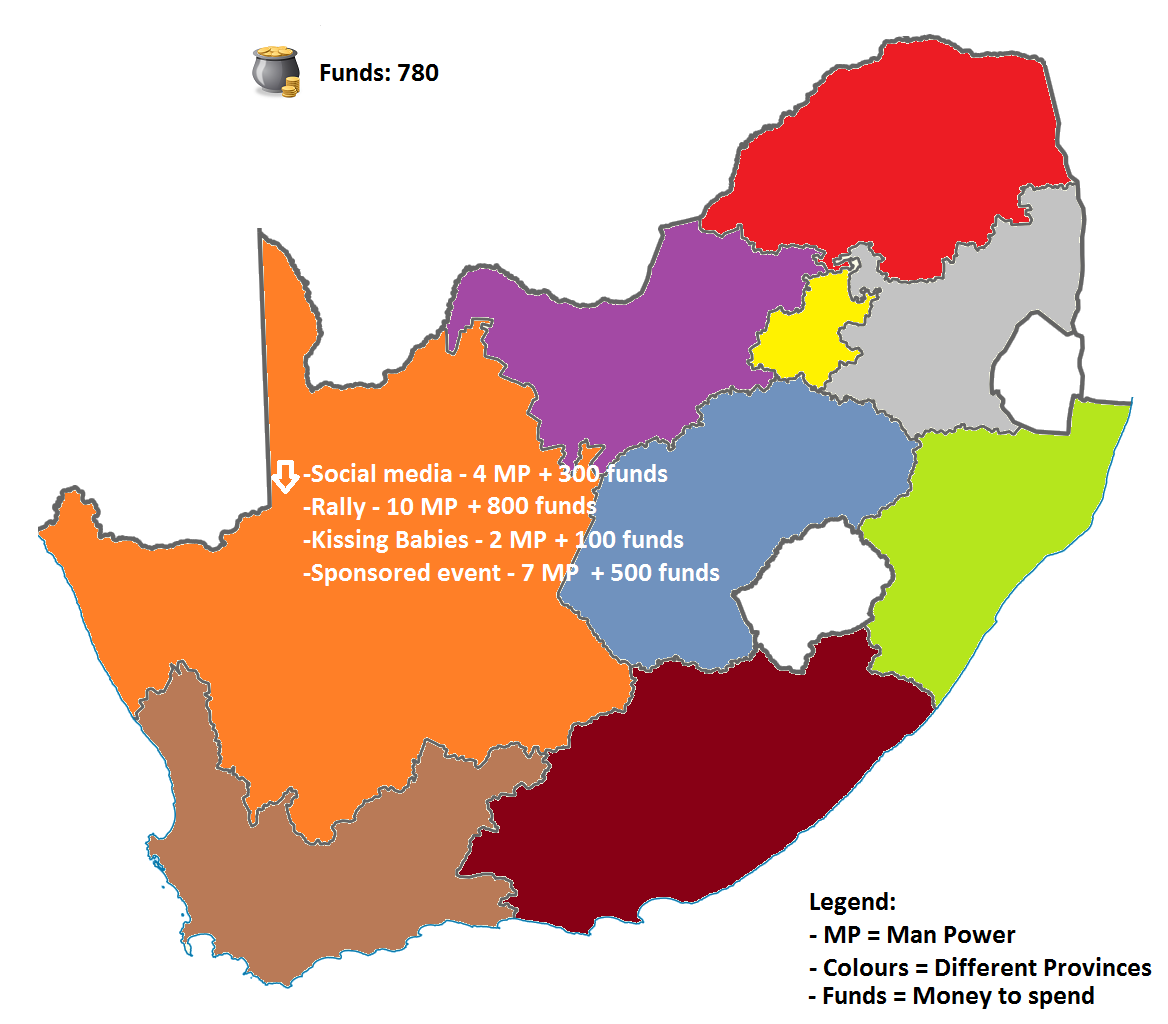
\includegraphics[width=1\linewidth]{Images/MAP.png}\\
\end{document}
